% Select language used in document (ngerman or english). Automatically
% generated text is translated accordingly.
% use \selectthesislanguage in body.tex to switch to default language

%\documentclass[ngerman, paper]{mmt} % use for BA1
\documentclass[english, bachelorthesis]{mmt} % use for BA2
%\documentclass[ngerman, masterthesis]{mmt} % use for Master thesis

\usepackage{mathptmx}
\usepackage{graphicx}
\usepackage{times}
\usepackage{subfig}
\usepackage{float}
\usepackage[utf8]{inputenc}
\usepackage{listings}
\usepackage{makecell}
\usepackage[toc,page]{appendix}
\usepackage{hyperref}
\hypersetup{
    colorlinks,
    citecolor=black,
    filecolor=black,
    linkcolor=black,
    urlcolor=black
}
\usepackage{breakurl}

\usepackage{amsmath}
\usepackage[autostyle,german=guillemets]{csquotes}

% moved to cls file. use \selectthesislanguage to switch to default language
%\usepackage[english,ngerman]{babel}

\usepackage{abbrevs}
%% the following solves a bug in the abbrevs package, that adds an empty
%% space after the abbrev
\makeatletter
\renewcommand\maybe@space@{%
  % \@tempswatrue % <= this is in the original
  \maybe@ictrue % <= this is new
  \expandafter   \@tfor
    \expandafter \reserved@a
    \expandafter :%
    \expandafter =%
                 \nospacelist
                 \do \t@st@ic
  % \if@tempswa % <= this is in the original
  \ifmaybe@ic % <= this is new
    \space
  \fi
}
\makeatother
%%


\usepackage{listings}
\usepackage{color}
\definecolor{lightgray}{rgb}{.9,.9,.9}
\definecolor{darkgray}{rgb}{.4,.4,.4}
\definecolor{purple}{rgb}{0.65, 0.12, 0.82}
\lstdefinelanguage{JavaScript}{
  keywords={break, case, catch, continue, debugger, default, delete, do, else, false, finally, for, function, if, in, instanceof, new, null, return, switch, this, throw, true, try, typeof, var, let, const, void, while, with},
  morecomment=[l]{//},
  morecomment=[s]{/*}{*/},
  morestring=[b]',
  morestring=[b]",
  ndkeywords={class, export, boolean, throw, implements, import, this},
  keywordstyle=\color{blue}\bfseries,
  ndkeywordstyle=\color{darkgray}\bfseries,
  identifierstyle=\color{black},
  commentstyle=\color{purple}\ttfamily,
  stringstyle=\color{red}\ttfamily,
  sensitive=true
}

\lstset{
   language=JavaScript,
   backgroundcolor=\color{lightgray},
   extendedchars=true,
   basicstyle=\footnotesize\ttfamily,
   showstringspaces=false,
   showspaces=false,
   numbers=left,
   numberstyle=\footnotesize,
   numbersep=9pt,
   tabsize=2,
   breaklines=true,
   showtabs=false,
   captionpos=b
}

\usepackage[authordate,bibencoding=auto,strict,noibid,backend=biber]{biblatex-chicago}
\bibliography{bibliography}

%% Add configuration options
\newabbrev{\authorname}{Marco Herzog}
\newabbrev{\authormail}{mherzog.mmt-b2017@fh-salzburg.ac.at}
\newabbrev{\titlename}{Using a virtual reality drunk driving simulator as an education tool for novice drivers}
\newabbrev{\advisor}{Dipl.-Ing. Dr.-Ing. Michael Domhardt}
%\newabbrev{\secondadvisor}{Titel Vorname Nachname}
\newabbrev{\thesisdate}{10.08.2020}
\newabbrev{\keywordsenglish}{virtual reality, driving simulation, alcohol, driver training, education}
\newabbrev{\keywordsgerman}{}


%% Paper title.

\title{\titlename}

%% This is how authors are specified in the conference style

%% Author 
\author{ \authorname\\ \scriptsize \authormail \\ \scriptsize 
\ifmmtlanguagegerman FH Salzburg \else Salzburg University of Applied Sciences \fi
}

%% A teaser figure can be included as follows, but is not recommended since
%% the space is now taken up by a full width abstract.
%\teaser{
%  \includegraphics[width=1.5in]{sample.eps}
%  \caption{This can be a teaser image of the thesis.}
%}

%% Abstract section for paper format.
\abstract{
    \ifmmtlanguagegerman 
        \selectlanguage{ngerman}
        Verkehrsunfälle und -vergehen im Zusammenhang mit Alkohol sind ein konstantes Problem im öffentlichen Straßenverkehr und Trunkenheit am Steuer wird häufig in der Fahrausbildung diskutiert.
Eine Reihe von Methoden versuchen die Menschen für die negativen Auswirkungen von Alkohol am Steuer zu sensibilisieren und schafften es diese Art von Verkehrsvergehen zu senken.
Trotzdem zeigt die Forschung, dass vor allem junge Erwachsene die Gefahren von Alkohol am Steuer unterschätzen und bessere Aufklärungsmaßnahmen benötigt werden. 
Mit der vermehrten Anwendung von virtuellen Simulationen in der Fahrerausbildung schlägt diese Arbeit einen Virtual Reality Fahrsimulator vor, der eine betrunkene Autofahrt simulieren soll.
Damit sollen Fahranfänger auf die Beeinträchtigung ihrer Fähigkeiten durch Alkohol aufmerksam gemacht werden und es soll als zusätzliches Werkzeug in der Führerscheinausbildung agieren.
Dazu wurde eine Studie in einer Fahrschule mit insgesamt 15 Fahrschülern durchgeführt.
Jeder Einzelne musste eine Sammlung von Aufgaben insgesamt zwei Mal durchführen, einmal mit simulierter Trunkenheit und einmal ohne zusätzliche Einschränkungen.
Die Auswirkung auf die Fahrfähigkeiten wurde durch die Reaktionszeit, die Spurhaltung und den Zeitaufwand für die Aufgaben gemessen.
Zusätzlich mussten die Teilnehmer einen Fragebogen ausfüllen, der die subjektive Meinung und Wahrnehmung feststellen sollte.
Die Auswertung beschäftigte sich mit den relativen Unterschieden jedes Teilnehmers sowie mit den Ergebnissen des Fragebogens.
Da keine relevanten Abweichungen von der normalen zur betrunkenen Fahrt festgestellt werden konnten, ist die Effektivität des Simulators nicht objektiv bestätigt.
Die Ergebnisse des Fragebogens zeigen hingegen eine positive Einstellung zur Simulation und zu dessen Bemühungen zur Aufklärung von Fahranfängern.  
Mit Qualitätsverbesserungen und weiteren Evaluierungen könnte der Fahrsimulator im Fahrschulunterricht als eine freiwillige Zusatzleistung verwendet werden.

    \else 
        \selectlanguage{english}
        Alcohol-related traffic violations and accidents are a constant problem in public traffic and drunk driving is a frequently discussed topic in basic driver training.
Various methods to sensitize people to the negative implications of driving under the influence of alcohol exist and managed to decrease the legal violations by a significant amount over the last years.
However, research shows that especially young adults tend to underestimate the dangers of drunk driving and more effective ways to impart the educational message are needed.
With virtual simulations being an accepted alternative to real-life driver training, this work proposes a virtual reality driving simulation that replicates alcohol intoxication to the user.
The aim of the simulator is to give novice drivers an understanding of the severe impact of alcohol on their driving capabilities.
Intended to be used as an addition to basic driver training, a study was conducted at a driving school with 15 participants, all of which were in training to get their driving license at that point.
Each subject was tasked to fulfil the same set of objectives two times, once with simulated drunkenness and once without any effects.
To measure the impact on the driving performance, the reaction time, the ability to stay within a given path and the time it took to finish the given tasks was recorded.
Additionally, a questionnaire was handed out to gather the subjective perception and opinion of the simulation.
The evaluation determined the relative performance changes of each subject and analysed the results of the questionnaire.
Since no significant deviations from the normal to the drunk run were observed, the effectiveness of the simulation could not be validated by the measured data.
The results of the questionnaire show a positive reception of the simulator and its educational intention.
With improvements on the quality and further evaluation, the use of a virtual reality drunk driving simulation could be a potential voluntary addition to basic driver training programs.

    \fi
}

%%%%%%%%%%%%%%%%%%%%%%%%%%%%%%%%%%%%%%%%%%%%%%%%%%%%%%%%%%%%%%%%
%%%%%%%%%%%%%%%%%%%%%% START OF THE PAPER %%%%%%%%%%%%%%%%%%%%%%
%%%%%%%%%%%%%%%%%%%%%%%%%%%%%%%%%%%%%%%%%%%%%%%%%%%%%%%%%%%%%%%%%

\begin{document}
% TODO switch for english, german
\selectthesislanguage

\pagenumbering{gobble}

 % group open
\ifmmtpaper 
\begingroup 
    % is required because paper template messes with sizes
    \fontsize{12}{18}\selectfont        
    \setlength{\parindent}{0pt}
    \setlength{\parskip}{5pt plus 2pt minus 1pt}
    \sectionfont{\fontsize{14}{15}\selectfont}
\fi

    \begin{titlepage}

% check if second advisor exists
\newcommand{\printsecondadvisor}[1]{%
  \ifcsname#1\endcsname%
  \ifmmtlanguagegerman ZweitbetreuerIn: \else Second Advisor: \fi \secondadvisor 
  \else%
    
  \fi%
}

\ifmmtmasterthesis

    
    % \begin{center}
    %     \Huge{ 
    %     	\textbf{\ifmmtlanguagegerman Masterarbeit \else Master Thesis \fi}
    %     }
    % \end{center}
    
    \newpage
    
    \thispagestyle{empty}
    
    \hfill \includegraphics[height=1.5cm]{images/FHSLogo.jpg}
    
    \vspace*{2cm}
    
    \Large{
    \titlename
    
    \vspace*{1cm}
    
    \ifmmtlanguagegerman
    Masterarbeit zur Erlangung des akademischen Grades
    \else
    Master thesis in partial fulfilment of the requirements for\\ the degree of 
    \fi
    
    \vspace*{0.5cm}
    
    \textit{Master of Science}
    }
    
    
    \vspace*{1.5cm}
    {\large
    \ifmmtlanguagegerman AutorIn: \else Author: \fi \authorname
    }
    \vfill
    
    {\normalsize
    \ifmmtlanguagegerman
    Vorgelegt am FH-Masterstudiengang MultiMediaTechnology, Fachhochschule Salzburg
    \else
    Submitted to the Master degree program MultiMediaTechnology, Salzburg University of Applied Sciences
    \fi
    
    
    \vspace*{1cm}
    
    \ifmmtlanguagegerman BetreuerIn: \else Advisor: \fi
    \advisor
    \\    
    \printsecondadvisor{secondadvisor}
    
    \vfill
    
    Salzburg, \ifmmtlanguagegerman Österreich, \else Austria, \fi  \thesisdate
    }

\else % Bachelor thesis title page

    \begin{center}
    
    \includegraphics[width=5cm]{images/FHSLogo.jpg}


    \vspace*{4cm}
    
    \fontsize{20.79}{18pt}{\selectfont        
    %\Large{
    	\textit{\textbf{\titlename}}
    %}
    }
    
    \vspace*{4cm}
    
    \fontsize{20.79}{18pt}{%\large{
    \ifmmtlanguagegerman
    	\textbf{Bachelorarbeit \ifmmtpaper 1 \else 2 \fi }
    \else
        \textbf{Bachelor Thesis \ifmmtpaper 1 \else 2 \fi }
    \fi
    }
    
    
    \end{center}
    
    \vfill
    
    %\begin{tabular}{ll}
    \ifmmtlanguagegerman AutorIn: \else Author: \fi  \authorname  \\
    \ifmmtlanguagegerman BetreuerIn: \else Advisor: \fi \advisor \\
    \printsecondadvisor{secondadvisor}
    
    Salzburg, \ifmmtlanguagegerman Österreich, \else Austria, \fi \thesisdate
    
    
    
    % uncomment the following 3 lines for an optional lock flag, max. 2 years!
    %\hfill
    %\color{red}
    %\framebox{Sperrvermerk bis 20/01/2012}

\fi

\end{titlepage}
        
    \onecolumn           
    
    \pagenumbering{roman}
    
    \newpage
    
\ifmmtlanguagegerman
\subsection*{Eidesstattliche Erklärung}


Ich erkläre hiermit eidesstattlich, dass  ich  die vorliegende Arbeit selbständig  und ohne fremde Hilfe verfasst, und keine  anderen  als die angegeben Quellen und  Hilfsmittel benutzt  habe. Weiter versichere ich hiermit, dass ich   die den benutzten Quellen  wörtlich oder inhaltlich entnommenen Stellen als solche kenntlich gemacht habe.

Die Arbeit wurde bisher in gleicher oder ähnlicher Form keiner anderen Prüfungskommission weder im In- noch im Ausland vorgelegt und auch nicht veröffentlicht.

\else

\subsection*{Affidavit}

I herewith declare on oath that I wrote the present thesis without the help of third persons and without using any other sources and means listed herein; I further declare that I observed the guidelines for scientific work in the quotation of all unprinted sources, printed literature and phrases and concepts taken either word for word or according to meaning from the Internet and that I referenced all sources accordingly.

This thesis has not been submitted as an exam paper of identical or similar form, either in Austria or abroad and corresponds to the paper graded by the assessors.

\fi

\vspace*{3cm}

%{\bf \thesisdate{}}


\hfill

\ifmmtlanguagegerman
$\overline{Datum \hspace{2cm}}$ \hfill $\overline{{Unterschrift}\hspace{3cm}}$

\vspace*{1cm}

\hfill $\overline{{Vorname\hspace{2cm}Nachname}}$
 
 \else
 $\overline{Date \hspace{2cm}}$ \hfill $\overline{{Signature}\hspace{4cm}}$

\vspace*{1cm}

 \hfill $\overline{{First~Name\hspace{2cm}Last~Name}}$
 \fi

  % comment out for expose

% group closing
\ifmmtpaper
\endgroup
\fi

%\ifmmtpaper\else
    
    \newpage
    \selectlanguage{ngerman}
    \section*{Kurzfassung}
    Verkehrsunfälle und -vergehen im Zusammenhang mit Alkohol sind ein konstantes Problem im öffentlichen Straßenverkehr und Trunkenheit am Steuer wird häufig in der Fahrausbildung diskutiert.
Eine Reihe von Methoden versuchen die Menschen für die negativen Auswirkungen von Alkohol am Steuer zu sensibilisieren und schafften es diese Art von Verkehrsvergehen zu senken.
Trotzdem zeigt die Forschung, dass vor allem junge Erwachsene die Gefahren von Alkohol am Steuer unterschätzen und bessere Aufklärungsmaßnahmen benötigt werden. 
Mit der vermehrten Anwendung von virtuellen Simulationen in der Fahrerausbildung schlägt diese Arbeit einen Virtual Reality Fahrsimulator vor, der eine betrunkene Autofahrt simulieren soll.
Damit sollen Fahranfänger auf die Beeinträchtigung ihrer Fähigkeiten durch Alkohol aufmerksam gemacht werden und es soll als zusätzliches Werkzeug in der Führerscheinausbildung agieren.
Dazu wurde eine Studie in einer Fahrschule mit insgesamt 15 Fahrschülern durchgeführt.
Jeder Einzelne musste eine Sammlung von Aufgaben insgesamt zwei Mal durchführen, einmal mit simulierter Trunkenheit und einmal ohne zusätzliche Einschränkungen.
Die Auswirkung auf die Fahrfähigkeiten wurde durch die Reaktionszeit, die Spurhaltung und den Zeitaufwand für die Aufgaben gemessen.
Zusätzlich mussten die Teilnehmer einen Fragebogen ausfüllen, der die subjektive Meinung und Wahrnehmung feststellen sollte.
Die Auswertung beschäftigte sich mit den relativen Unterschieden jedes Teilnehmers sowie mit den Ergebnissen des Fragebogens.
Da keine relevanten Abweichungen von der normalen zur betrunkenen Fahrt festgestellt werden konnten, ist die Effektivität des Simulators nicht objektiv bestätigt.
Die Ergebnisse des Fragebogens zeigen hingegen eine positive Einstellung zur Simulation und zu dessen Bemühungen zur Aufklärung von Fahranfängern.  
Mit Qualitätsverbesserungen und weiteren Evaluierungen könnte der Fahrsimulator im Fahrschulunterricht als eine freiwillige Zusatzleistung verwendet werden.

    \ifmmtmasterthesis
    
    \vspace*{0.5cm} 
    \textbf{Schlüsselwörter:~} \keywordsgerman
    \fi
    \newpage
    \selectlanguage{english}
    \section*{Abstract}
    Alcohol-related traffic violations and accidents are a constant problem in public traffic and drunk driving is a frequently discussed topic in basic driver training.
Various methods to sensitize people to the negative implications of driving under the influence of alcohol exist and managed to decrease the legal violations by a significant amount over the last years.
However, research shows that especially young adults tend to underestimate the dangers of drunk driving and more effective ways to impart the educational message are needed.
With virtual simulations being an accepted alternative to real-life driver training, this work proposes a virtual reality driving simulation that replicates alcohol intoxication to the user.
The aim of the simulator is to give novice drivers an understanding of the severe impact of alcohol on their driving capabilities.
Intended to be used as an addition to basic driver training, a study was conducted at a driving school with 15 participants, all of which were in training to get their driving license at that point.
Each subject was tasked to fulfil the same set of objectives two times, once with simulated drunkenness and once without any effects.
To measure the impact on the driving performance, the reaction time, the ability to stay within a given path and the time it took to finish the given tasks was recorded.
Additionally, a questionnaire was handed out to gather the subjective perception and opinion of the simulation.
The evaluation determined the relative performance changes of each subject and analysed the results of the questionnaire.
Since no significant deviations from the normal to the drunk run were observed, the effectiveness of the simulation could not be validated by the measured data.
The results of the questionnaire show a positive reception of the simulator and its educational intention.
With improvements on the quality and further evaluation, the use of a virtual reality drunk driving simulation could be a potential voluntary addition to basic driver training programs.

    \ifmmtmasterthesis
        
    \vspace*{0.5cm} 
    \textbf{Keywords:~} \keywordsenglish
    \fi
    \selectthesislanguage
    
    \newpage
    \tableofcontents
    
    \newpage
    \ifmmtlanguagegerman
\section*{Abkürzungsverzeichnis}
\else
\section*{Abbreviations}
\fi

\begin{table}[h]		
	\begin{tabular}{ll}
		BAL & Blood alcohol level \\
		VR & Virtual reality \\
		LCT & Lane change test \\
		HMD & Head mounted display \\
		URP & Univeral render pipeline \\
		LOS & Line of sight \\
		SUV & Sports utility vehicle \\
		CSV & comma separated value \\
		

		
	\end{tabular}
\end{table}

    \listoffigures
    % \lstlistoflistings
    \listoftables
    
%\fi

\mmtcolumnmode % switch back to column formatting of stylesheet

\maketitle % used for paper formatting

\ifmmtpaper\else
\pagestyle{headings}
\fi
\pagenumbering{arabic}


%for reference to this section
\section{Introduction}
\label{section:Introduction}
Driving under the influence of alcohol is a constantly observed traffic violation and a contributing factor for many traffic accidents in Europe \autocite[]{fell2014update}.
This behaviour is especially common for adolescents \autocite[]{arnett1990drunk} and is an integral part in the theoretical teaching plan in Austrian driving schools  \footnote{http://www.bos.at/ebook/probe/fw/b/44/}.
This includes basic information on how the blood alcohol level (BAL) is affected, the common effects of alcohol on the driver and the legal framework.
Considering the data on traffic violations in Austria regarding drunk drivers \autocite[107]{bmasgk2019alkohol} a decline in criminal charges is observed in recent years.
This improvement can be linked to more frequent traffic controls and stricter legal limits for the BAL. 
Also, educators are utilising different methods, e.g. shocking imagery and stories \footnote{http://www.close-to.net/} or specifically designed googles \footnote{https://www.fatalvision.com/}, to sensitize people to the implications of alcohol.
Nevertheless, a significant number of people are known to have driven under the influence of alcohol, with most of them being well aware on the implications on their abilities and possible consequences of their actions \autocite[]{alonso2015driving}.
To this date it is still of high relevance to properly educate drivers about the dangers of drunk driving and find new ways to impart this knowledge, especially to novice drivers.
\\
With the advance of digital simulations and their acceptance as serious learning tools \autocite[]{backlund2006computer}, many advantages to real-life training can be determined. 
Illegal or dangerous traffic situations can be reproduced and trained multiple times and are known to positively impact the learning effect when executed right \autocite[]{vlakveld2005use}.
Using Virtual Reality (VR), the immersion of driving simulators can be enhanced significantly \autocite[498]{ihemedu2015development}, which is argued to be an important factor in the quality of a simulation designed for training. \autocite[2]{vlakveld2005use}
The improved effectiveness of VR based learning environments is evaluated by \textcite{chen2006design} and is argued to be better than conventional non-VR learning software. 
An implementation of a VR driving simulation that replicates an alcohol intoxicated car ride was tested by \textcite[]{von2016cyber} and could potentially be adopted to use in driver education.
Without any major risk this would allow educators to teach the implications of alcohol on driver abilities in an engaging way. 
\\
Aim of this work is to develop such a drunk driving simulation in VR and to evaluate its potential use in basic driver training.
The drunk driving simulator is supposed to severely impact the driver abilities and create a lasting experience to sensitize the user to the negative implications of driving drunk.
Geared towards the use in driving schools with minimal cost and space requirements, commonly available equipment and technology is used for the development. 
Possible ways to create an authentic replication of alcohol intoxication are explored and tested in a laboratory experiment.
The study is held at an Austrian driving school with 15 novice drivers as test subjects.
Three different sets of objective measurements are supposed to identify any relative deviations in driver behaviour when driving in the same simulator with and without the proposed simulated drunkenness.
These measurements include the reaction time, the ability to stay within a given path and the overall time to finish the car drive.
This data is then statistically evaluated to potentially validate the negative effect of the drunk driving simulation on driver abilities.
While reaction time is expected to increase and viewed separately, the ability to stay within a path, which is supposed to deteriorate, and the time to finish is evaluated together to find potential relations. 
A questionnaire after the experiment is conducted to gather feedback on the simulation as well as to subjectively determine the acceptance as a serious learning tool in basic driver training.
Finally, the outcome of the study is discussed and an outlook for future work is given. 





\section{Related work}
\label{section:relatedWork}
The following section analyses scientific literature and statistics to show the need for the proposed drunk driving simulator as well as to provide a theoretical base to build a plausible simulation and to conduct a statistically sound user evaluation.
In section \ref{subsection:drunkDriving} the current state of drunk driving violations is viewed, while section \ref{subsection:alcoholEducation} identifies methods used to educate drivers on the impact of alcohol intoxication.
Section \ref{section:driver training} gathers information about simulations and their use in practice, section \ref{subsection:effects of alcohol} views the medical implications of alcohol on bodily functions and section \ref{section:measurePerformance} determines possible ways to measure the driver performance in a virtual simulation.


%
%###########################################
\subsection{Drunk Driving}
\label{subsection:drunkDriving}
%
%###########################################
Recent reports have shown that driving under the influence of alcohol is a major risk factor in many traffic accidents in Europe. \autocite{fell2014update}
\\
A frequently updated analysis on behalf of the Austrian Federal Ministry of work, social issues, health and consumer protection \autocite[107]{bmasgk2019alkohol} collects and evaluates alcohol-related statistics in Austria reaching back several decades.
Since 1998, when the criminal limit of the BAL was lowered from 0.8 to 0.5 in Austria, a major decrease in fines related to this offense as well as an increase in traffic controls was observed.
The authors conclude a significant decline in drunk drivers from this year on.
However, taking the data on traffic accidents with the involvement of alcohol intoxicated drivers into consideration, no substantial changes in accidents and injured persons is observed since 2012.
From 2012 to 2018 an average of 6.23\% (SD: 0.22\%) of all recorded traffic accidents with personal injuries were accidents with at least one participant being under the influence of alcohol.
In the same context an average 6.4\% (SD: 0.22\%) of injured persons were also involved in these types of accidents. 
\\
In a statistical report on traffic accidents in Germany of 2018 \autocite[]{destatis2019alkohol} a similar trend can be observed.
While the overall number of convicted drunk drivers decreased by 17.57\% from 2012 to 2017 \autocite[51]{destatis2019alkohol}, the involvement in traffic accidents in the same time period is constantly high.
It was determined that alcohol inebriated drivers were involved in 4.5\% of all accidents with personal injuries in 2018. 
7.5\% of all traffic fatalities were caused as a result of accidents where at least one participant was under the influence of alcohol.
According to this distribution alcohol induced traffic accidents tend to be much more severe.
The report further shows that 17.2\% of inebriated participants were between the age of 18 and 24 and 24.9\% were between 25 and 34 years old.
\\
In a collaborative study from 2019 of multiple Austrian institutes for traffic psychology \autocite[]{bartl2019alkohol}, 500 convicted drunk drivers were interviewed.
The study subjects were obligated to do a retraining course after they were caught driving under the influence of alcohol. 
The purpose of the retraining is to change the attitude towards drunk driving of each individual. 
33.5\% of the interviewees were involved in an accident. 
When asked what the person was thinking before getting into the car, 39.7\% believed that they were still able to drive.
The authors of the study also estimate that for each drunk driver that is caught during a police check, there are two inebriated drivers undetected.
\\
\textcite[1]{alonso2015driving} conducted a study to investigate the attitude towards driving under the influence of alcohol.
The results show that about a quarter of the interviewed participants admit to have driven drunk at least once.
The major motivation for this behaviour was the lack of alternative transportation and alcohol consumption related to meals. 
12.7\% of the interviewees with drunk driving experience on the other hand stated that they believe alcohol has no negative effects on their abilities.
%
%###########################################
\subsection{Alcohol education}
\label{subsection:alcoholEducation}
%
%###########################################

In the training of novice drivers, the theoretical implications of alcohol are taught and a fixed part in the teaching plan \footnote{http://www.bos.at/ebook/probe/fw/b/44/}.
Additionally, instructors tend to use graphic and shocking videos to visualize the possible outcomes of drunk driving.
There are also existing programs \footnote{http://www.close-to.net/}, in which convicted traffic offenders including drunk drivers visit driving schools and talk to students about their crimes and accidents.
Even though this makes novice drivers aware of the consequences, it does not convey the impact on their abilities even if just a small amount of alcohol is consumed.
Other methods to simulate alcohol intoxication are special googles that alter the vision of its users \footnote{https://www.fatalvision.com/}.
Certain tasks have to be performed while wearing these googles which are supposed to sensitize the users to the impairment caused by alcohol and other substances.
\\
As part of an project by a Chinese company \footnote{https://ifworlddesignguide.com/entry/246877-vr-drunk-driving-simulator} a similar VR simulation to the one in this work is developed.
This product aims to replicate a drunk drive to experience the negative effects of alcohol and is targeted for public use.
At the time of writing no further information to this project was found.


%
%###########################################
\subsection{Driver training with simulations}
\label{section:driver training}
%
%###########################################

\textcite[1]{vlakveld2005use} points out several advantages of a driver training simulation over driving lessons in real-life traffic situations.
The instructor has full control over the training conditions and is able to repeat and rehearse a given task as often as needed.
Dangerous situations can be practiced without any risk for the driver or his environment, which opens up the possibility to simulate scenarios that are very difficult to create in public traffic.
The trainees can also be provided with more detailed feedback since a computer-based simulation allows measuring of a wide variety of data e.g. speed, reaction times etc.
Even though these advantages enable the training of specific skills in isolated environments, it is uncertain if the learned skills can be applied in real traffic situations. 
According to \textcite[2]{vlakveld2005use} this is dependent on the quality of the simulation and a proper imitation of reality. 
The author suggests a combination with other training methods and devices to ensure the effectiveness of the simulator.
\\
The work of \textcite{waller1998transfer} confirms the importance of a realistic experience to achieve the best possible learning effect.
In theory, a perfect representation of a real-world environment in a training simulation would have the same learning impact as real-world training.
In case of a driving simulation this requires an authentic replication of a vehicle and its response to user input as well as a realistic surrounding area \autocite[130]{waller1998transfer}.
\\
A common issue observed in simulations, is the occurrence of the so-called simulation sickness \autocite[]{hettinger1992visually}.
Differences in perceived motion without actual physical movement may cause the affected person to experience a feeling of nausea. 
Another cause can be a significant delay between user input and the corresponding feedback coming from the simulation \autocite[2]{kemeny2014driving}.
To test the implications of simulation sickness on user enjoyment, \textcite{von2016cyber} developed and tested a VR racing game that tries to simulate the negative effects of alcohol on the human body by adding visual and auditive effects and distortion. 
Not contributing any scientific relevant findings, the authors conclude that the occurring sickness does not necessarily render a VR simulation useless.
\\
Depending on the requirements the driving simulator has to fulfil, some simplifications to the simulation have to be made to reduce the overall effort and costs during the development. 
These restrictions have further impact on the behaviour of its users but does not invalidate the use of simulators in driver training.  
Instead this requires instructors to carefully integrate the simulation into their training program. \autocite[3]{leitao1999evaluation} 
\\
In practice special equipment is available that is geared towards basic driver training and is mainly used in and by driving schools. 
An installation representing a car interior with all vital controls (pedals, gear box, steering wheel etc.) as well as multiple screens is available for purchase and has seen use in driving schools. \footnote{https://www.degener.de/produkt-kategorie/fahrschulunterricht/fahrsimulator/}
This simulation can be enhanced with a VR headset and several other modules to replicate difficult and dangerous situations in public traffic. 
\\


%
%###########################################
\subsection{Effects of alcohol intoxication}
\label{subsection:effects of alcohol}
%
%###########################################

In the following section a variety of research on the implications of ethanol intoxication is evaluated for the use in a virtual reality simulation. 
This includes especially changes in vision as well as general motor skills. 
For the purposes of this paper only a few characteristics of the influence of alcohol on human abilities can be simulated in a virtual environment. 
\\
\textbf{Reaction time} - It is known that the consumption of alcohol negatively affects the capability to process information and increases the reaction time (RT) \autocite[]{maylor1993alcohol}.
The implication on RT increases linearly with longer and/or more complex tasks.
\\
\textbf{Inattentional blindness} - A commonly observed phenomenon in scientific research as well as in practice is known as inattentional blindness \autocite[]{clifasefi2006blind}.
People tend to miss unexpected object or events in their field of vision when their attention is focused on something specific.
In a study held by \textcite{simons1999gorillas}, the participants were tasked to watch a video and count the number of passes in a basketball game. 
About the half of the participants failed to notice a man in a full gorilla costume that was also acting in the scene.
\textcite{clifasefi2006blind} evaluated the influence of alcohol on inattentional blindness with the same video as above and came to the conclusion that even small amounts increase the occurrence of this phenomenon. 
The authors link this outcome to a model named \textbf{alcohol myopia}.
It causes intoxicated individuals to focus more attention as usual to more prominent events and lose awareness for other details in their peripherals. \autocite{steele1990alcohol}
Since the participants were asked to perform a certain task (counting), the attention was drawn to the events regarding this task. 
In the context of driving a vehicle an example would be focusing on staying in lane and missing a pedestrian walking on the road.
\\
In a similar evaluation by \textcite{do2007effects} the control of visual attention under the influence of alcohol is observed. 
Participants were setup in an eye tracking system and were given tasks on where to focus their visual attention.
The difficulty of the tests varied and was divided into a simple and a more demanding task.
Results show that with a higher difficulty the subjects are less likely to be distracted by other events in their vision, a finding consistent with alcohol myopia. 
With a lower difficulty the attention tends to shift to other events and objects, the intoxicated subjects were less capable of ignoring distracting factors. 
The authors argue that this is related to the fact that alcohol decreases the ability to divide the attention in general \autocite{i1999effects}.
\\
\textbf{Vergence} - Alcohol is known to affect the vergence, the ability to move both eyes in opposite directions to achieve binocular vision \autocite{cassin1984dictionary}.
It reduces the limits in which the intoxicated person can fuse the perceived stereo images into a single three-dimensional image. 
In their study \textcite{miller1991effect} have shown that people under the influence of alcohol tend to experience diplopia for further away targets.
Diplopia is simultaneous perception of two images of the same object that are displaced vertically, horizontally, diagonally or rationally. \autocite[]{cassin1984dictionary}
A higher BAL will decrease the distance in which the person can see without diplopia for near and far targets.
For driving this might cause difficulties when trying to identify road signs and other traffic participants as well as trying to identify crucial information on the driver’s dashboard. 
The time required to fuse the perceived stereo images, also known as fusion latency, is increased for near and far targets. 
At intermediate distances the fusion latency was not affected by alcohol intoxication.
\\
\textbf{Eye movement} - The work of \textcite{moser1998effect} investigates the effect of alcohol on eye movement.
Smooth-pursuit eye movements, the ability to follow moving objects up to a certain velocity, are impaired for intoxicated people when tracking targets that are moving with a constant velocity. 
The decreased ability to pursuit movement is compensated by an increased number of catch-up \textbf{saccades} which are quick, simultaneous movements of both eyes between multiple fixation points \autocite{cassin1984dictionary}.
The velocity and latencies of saccadic eye movements is also decreased with a higher BAL.
There is no significant change in the accuracy of the saccades.
Intoxicated people show longer fixation duration and a reduced number of exploratory saccades when scanning a specific scenery.
The authors claim that the intoxication causes a deficit in understanding and processing the information of the fixated area.
\\
\textbf{Contrast sensitivity} - Even small doses of alcohol are known to reduce the contrast sensitivity for stationary and moving targets \autocite{nicholson1995effects}.
Contrast sensitivity can be described as the ability to distinguish lighter and darker areas in a perceived image.
\textcite[]{nicholson1995effects} mention that the impact on the visual performance on the contrast sensitivity was greater for moving targets. 
\\
\textbf{Balance} - A known effect of alcohol is a negative effect on the sense of balance \autocite{nieschalk1999effects}.
The intoxication tends to increase the postural sway and negatively affects the ability to coordinate the postural movement with voluntary activities. 
In their study, \textcite{nieschalk1999effects} find that with high BAL ($>$ 0.8‰) the body sway is increased significantly. 
With a lower percentage the sway is not as severe, but the authors mention that a stable posture is also influenced by psychological factors.
Since the test subject were aware of the aim of the study and were asked to perform to the best of their abilities, the results with low BAL might not reflect the actual impact. 
The authors also observed an improvement to the postural sway of certain subjects after consuming small doses of alcohol. 
\textcite{nieschalk1999effects} argue that this may be related to the stimulating effect that small doses of alcohol have on psychomotorical abilities and therefore improve overall performance.



%
%###########################################
\subsection{Measuring driver performance}
\label{section:measurePerformance}
%
%###########################################
Many personal factors, such as fatigue, stress, experience etc., influence every individual differently and are generally difficult to assess in a statistical manner. \autocite[16]{jurecki2011test}
In the following sections the possible ways to get objective measurements for driving performance are researched and evaluated.
\\

\subsubsection{Lateral position}
\label{subsection:lateral position}
A very commonly used metric to define driving behaviour is lateral positioning. \autocite[37]{ostlund2005driving}
It measures the driver’s ability to stay within a safe path and is influenced by many factors like driving experience, distraction and road environment.
It is common to use a straight road with multiple lanes while the user has to stay within the lane as precisely as possible \autocite[]{iso201026022} \autocite[]{brouwer1991divided}.
\\
A standardized test known as the "lane change test" (LCT) \autocite[]{iso201026022} is used to measure the impact on the drivers abilities when performing two tasks simultaneously.
The primary objective is to drive along a straight road with three lanes with a constant speed.
In regular intervals signs are appearing near the road and the users are instructed to change the lane according to the signal.
The vehicle properties are tracked with minimum sampling rate of 10 Hz during the experiment e.g. position on track, steer angle etc.
Even though this test is mainly used to measure the driver distraction by the secondary task, the path deviation measurement can still be used for the tracking test in this study.
As seen in figure \ref{figure:LCTNormative} this model can be used to identify the average deviation from the ideal path and is calculated as follows: \autocite[13]{iso201026022}
\begin{equation}
\label{equation:LCTMeanDeviation}
	\frac{1}{S}\sum[x_{deviation},i(\frac{y_{i+1}-y_{i-1}}{2})]
\end{equation}
\begin{equation}
\label{equation:deviation}
    x_{deviation,i} = |x_{position,i} - x_{reference,i}|
\end{equation}

\begin{figure}[h]
    \centering
	\includegraphics[width=1\linewidth]{images/lctNormativeModel.png}
	\caption[
		LCT normative model
	]{
		Standard analysis of LCT \autocite[77]{ostlund2005driving}
	}
	\label{figure:LCTNormative}
\end{figure}

The variables $x_{position,i}$ and $x_{reference,i}$ describe the lateral position of the vehicle on the track.
$x_{deviation,i}$ is the lateral deviation, $S$ the amount of data segments and $y$ the longitudinal position on the track.
\\

% The LCT is
% In a study to evaluate the differences in the driving capabilities of young and old drivers, \textcite[576]{brouwer1991divided} used a similar method as explained above.
% The subjects were tasked to continuously follow a straight road while a variable force pushed the vehicle to left or right.
% During the experiment a secondary assignment was given to the participants to determine the driving performance with divided attention.
% The amount of time the users were able to stay within their lane is described as "time on target". 
% To find the relative performance
% \\

\subsubsection{Reaction time}
\label{subsection:reaction time}

In the context of driving, reaction time is an important parameter in designing safe roads \autocite[195]{green2000long} and in the analysis of traffic accidents. \autocite[]{jurecki2011test}
\\
Even though there are established norms on the average reaction times, many estimates in known literature are differing significantly from the standardized values. \autocite[]{green2000long} 
Literature reviews regarding the reaction times of driver’s state, that the main reason behind these discrepancies are the different testing conditions used by the researchers. \autocite[]{green2000long} \autocite[]{jurecki2011test}
\\
In their work \textcite[]{jurecki2011test} review the methods for determining reaction times while driving a vehicle.
Many of the analysed studies use simple cues like single lights or tones as a signal for the driver to react to.
The author states that in real traffic situations the indicators on when the driver should e.g. brake are much more complex.
In most cases additional actions are required to e.g. avoid a crash than just braking which further impacts the driver’s behaviour.
More realistic obstacles like inflatable car dummies \autocite[203]{jansson2002decision} try to simulate complex stimuli and are more popular in recent study reports. \autocite[17]{jurecki2011test}
It has to be noted that many of the above-mentioned tests were not held in virtual driving simulations but on test tracks or real roads.
As discussed in section \ref{section:driver training}, the use of a virtual environment allows for a more authentic scenario to evaluate the reaction times of the user as well as for an easy way to get exact measurements.
\\
For a better understanding reaction time can be separated into multiple components. \autocite[]{boff1988engineering}.
The time needed for perceiving a signal or object and deciding on a response is known as the "mental processing time".
In the proposed simulator this is the time the user needs for spotting the dummy, realizing it is moving towards the road and deciding to brake to avoid a collision.
The time it takes for the driver to move his foot away from the accelerator and pushing the brake pedal is known as "movement time".
The "device response time" is the amount of time the vehicle requires to perform the requested action e.g. the time it takes to fully stop the car.
\\
As \textcite[200]{green2000long} states that the mental processing time is the truest form of reaction time but many studies include the other mentioned components in their estimations.
Since the mental processing time is quite difficult to measure objectively without a physical response the test setup in this work also includes the movement time when evaluating the reaction time.
The device response time will not be included in the measurement because it does not contribute any valuable information to the purposes of this study.



\section{Implementation}
\label{section:implementation}
The implementation of the drunk driving simulator is realised with the Unity Engine 3D (Version 2019.4.5f1).
It offers a scripting API in C\#, which is used extensively in the development of the simulation. 
The accessible editor and the built-in asset store allow for quick prototyping with relatively low effort and cost.
The Unity asset store offers a wide variety of content e.g. 3D models, shades, textures, animations etc.
Many third-party assets are used to reduce the development time and create an engaging and visually appealing experience. 
All the used resources are listed and described in sections \ref{subsection:virtual environment}, \ref{subsection:input and physics} and \ref{subsection:visual effects}.
\\
The drunk driving simulator is loosely based on a similar bachelor thesis by \textcite{birgmann2018simulation}.
In this work a virtual reality simulation was developed to show the dangerous implications of distracting factors like using a phone when driving a vehicle.
Some of the assets used are recycled for the simulator in this work and are also listed in the above-mentioned sections.
\\
To simulate alcohol intoxication in VR, this work focuses solely on the effects on human vision and tries to replicate the implications as authentically as possible.
Other negative effects on e.g. balance are not implemented in the drunk driving simulator because of technical limitations and the occurrence of unbearable simulation sickness.
Possible and failed approaches to simulate drunkenness beyond visual effects are established in the discussion section of this work.
In section \ref{subsection:effects of alcohol} commonly observed implications on human abilities are researched and explained.
Section \ref{subsection:visual effects} describes the process on how these effects are implemented into the simulation.
\\
For the purposes of this study some additional logic is implemented to evaluate the behaviour and performance of each driver individually and how the proposed drunk driving simulator is affecting these characteristics.
To acquire usable data the participants of the study have to focus on two separate tasks that are supposed to reliably track their driving performance.
The first assignment is to follow a route along the road and keep the vehicle as close as possible to this path.
In predefined intervals the deviation from the ideal path is measured and logged.
In section \ref{subsection:tracking test} the exact setup of this test is explained.
\\
The second task given to the users is to watch out for potential jaywalkers and react to them by braking and evading if necessary.
This task is used to determine the reaction time of the participant and is elaborated in section \ref{subsection:reaction test}.

\subsection{Virtual Reality}

The virtual reality device used for this project is the Oculus Quest.
The head mounted display (HMD) is designed to provide a wireless VR experience but can also be used in combination with a stationary PC as well.
To use VR in Unity the Steam VR plugin \footnote{https://assetstore.unity.com/packages/tools/integration/steamvr-plugin-32647} has to be integrated into the engine.
The plugin provides a camera setup that can be placed in the scene and is fully functional without any major configurations. 

\subsection{Virtual Environment}
\label{subsection:virtual environment}


When designing the virtual environment several factors are taken into account.
The most important factor are the technical limitations that were present during development.
In his bachelor thesis, \textcite[]{birgmann2018simulation} reported major performance difficulties during the development of the simulation.
The surrounding area was a dense town with many buildings, traffic and other props to enhance the realism.
To meet a consistent and high frame-per-second count many modifications to the objects level of detail and culling properties had to be made that were not ideal.
\\
For the drunk driving simulator another performance concern has to be considered.
Since the drunkenness is mainly achieved through screen shaders that required the software to do additional render passes each frame, the hardware requirements are even higher.
For this reason, an environment with less objects and visual clutter was designed to avoid performance issues. (see figure \ref{figure:overviewEnvironment})
\\
The reason for the more rural appearance of the surroundings is the common traffic situation that is encountered in the place where the study is held.
Near the driving school most roads tend to be curvy and narrow and are surrounded by mostly woods, fields and sparsely populated urban areas.
Most of the study participants are known to be living in this area and are more accommodated to this type of environment.



\begin{figure}[h]
    \centering
	\includegraphics[width=1\linewidth]{images/overviewEnvironment.png}
	\caption[
		Simulator environment overview
	]{
		An overview of the simulator environment.
	}
	\label{figure:overviewEnvironment}
\end{figure}


The buildings scattered in the area are taken from the Town Constructor 3 asset pack. \footnote{https://assetstore.unity.com/packages/3d/environments/urban/town-constructor-3-71070}
It contains a variety of predefined buildings with different level of details that are changed during run-time, depending on the distance to the user camera.
This positively affects the performance since far away objects do not require as much computational power.
The road itself is made with the help of the EasyRoads3D Free v3 asset pack. \footnote{https://assetstore.unity.com/packages/3d/characters/easyroads3d-free-v3-987}
With custom editing tools the road can be easily created and modified and it automatically conforms the terrain to fit accordingly.
The entire track is arranged as a circuit to allow the user to drive multiple laps without a transition.
The terrain and the trees are placed with a built-in Unity functionality.
\\
The vehicle controlled by the user is taken from the realistic car HD 3 asset pack \footnote{https://assetstore.unity.com/packages/3d/vehicles/land/realistic-car-hd-03-113200} and resembles a small sport utility vehicle (SUV) with detailed interior and exterior. 

\subsection{User Input and Physics}
\label{subsection:input and physics}

The input devices used for the simulation is a Logitech G27 steering wheel with a set of pedals. 
With a built-in force feedback mechanism, the steering wheel handles authentically and works with the Unity input system without any issues.
For the physics and control of the vehicle the Realistic Car Controller asset pack \footnote{https://assetstore.unity.com/packages/tools/physics/realistic-car-controller-16296} is used.
The scripts in this pack provide a realistic vehicle control system that handles user input and allows for detailed configuration of the vehicle behaviour.
Most of the settings for the controlled car are taken over from the project of \textcite[]{birgmann2018simulation} since the same input setup was used in this simulation. 


\begin{figure}[h]
    \centering
	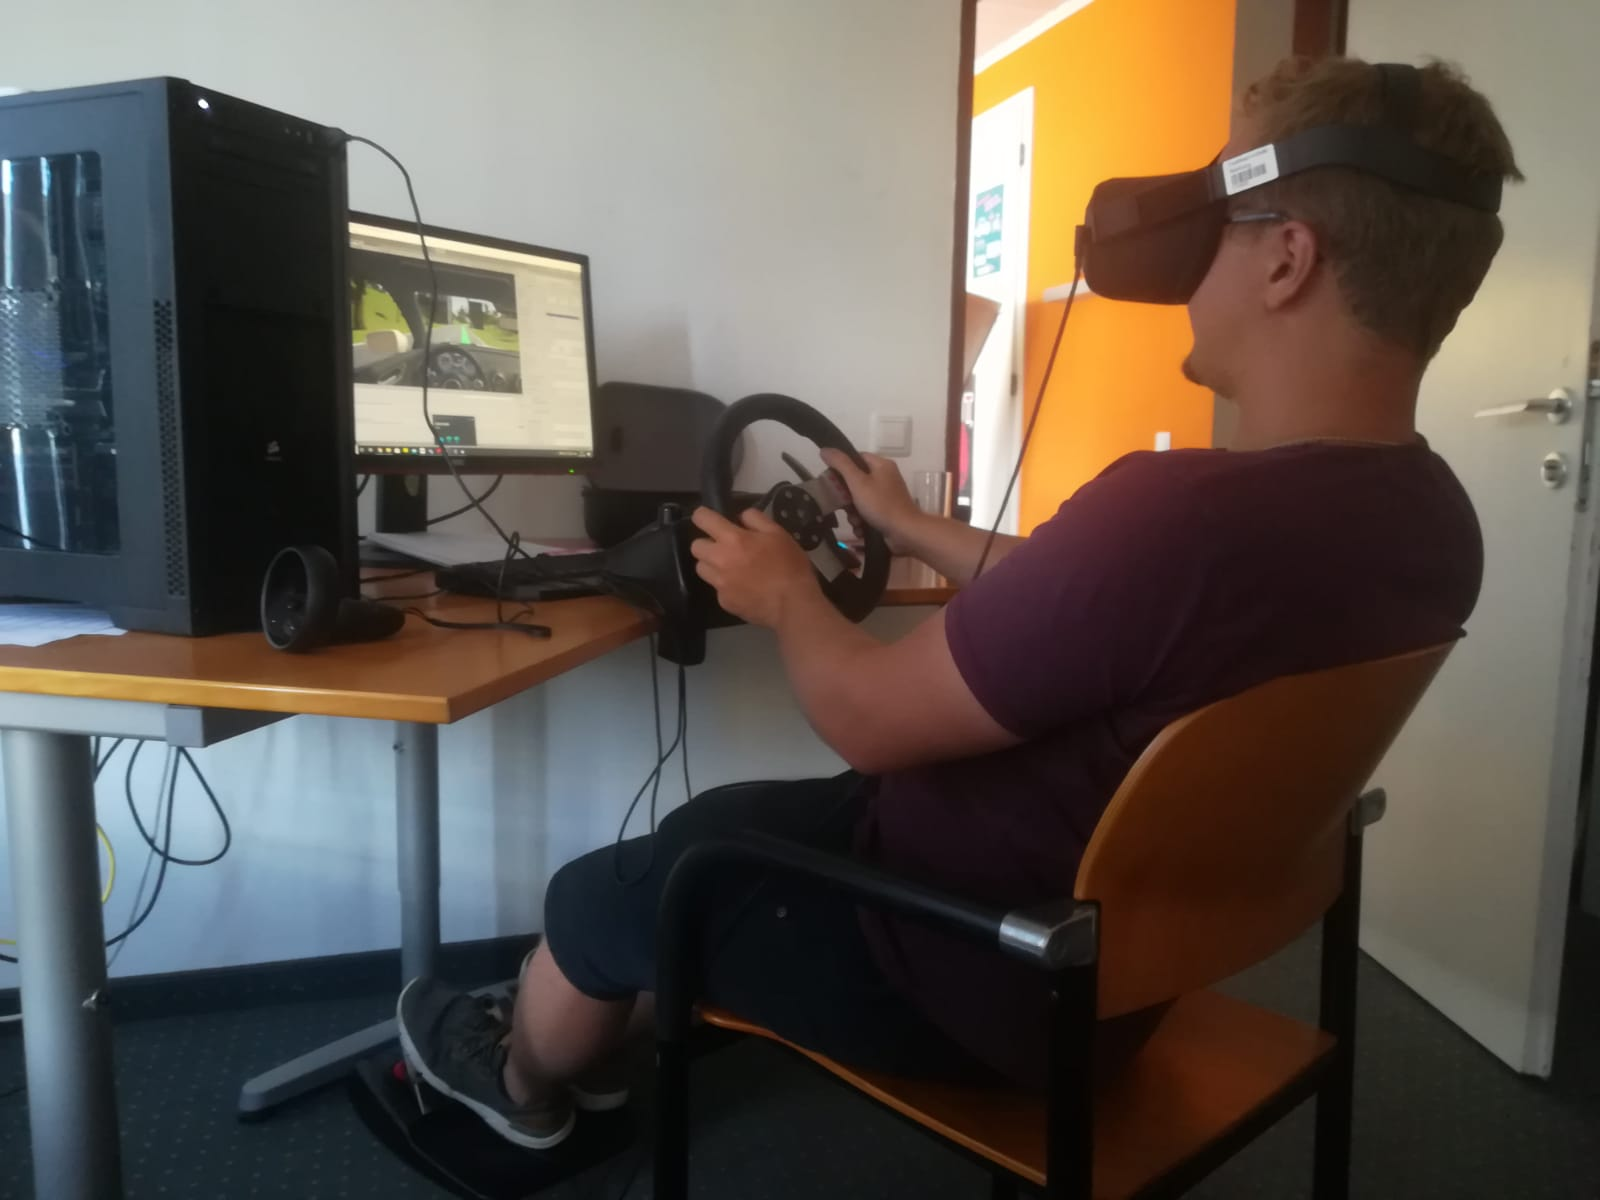
\includegraphics[width=1\linewidth]{images/studySetup.jpeg}
	\caption[
		Simulator setup
	]{
		Setup of the drunk driving simulator.
	}
	\label{figure:overviewEnvironment}
\end{figure}

\subsection{Visual effects}
\label{subsection:visual effects}

To create an authentic drunk experience in the VR simulation the Drunk Man asset pack \footnote{https://assetstore.unity.com/packages/vfx/shaders/fullscreen-camera-effects/drunk-man-47438} is used and modified to fit the needs of the evaluation.
The asset pack includes a camera shader that is supposed to simulate the vision of a drunk person and is generating multiple effects e.g. distortions, color shift, ghost vision etc.
Applying this shader to the camera requires the render pipeline to compute six additional render passes and affects the overall performance and visual quality.
A very noticeable side effect of the shader is the deactivation of anisotropic filtering when viewing the scene in VR.
Anisotropic filtering is supposed to eliminate aliasing effects \autocite{blinn1976texture} and in this case smooth the edges of textures to make their appearance less "blocky".
Even though this does not have implications on the course of the study, improvements on the effects are desirable and are further examined in the discussion section.
\\
Another issue is the amplified occurrence of simulator sickness when applying the shader in VR.
The asset pack is not designed for the use in VR and has to be altered and toned down to make it more tolerable.
To still achieve a decent drunk effect a script is attached to the camera that modifies the shader parameters dynamically according to the behaviour of the user.
To simulate the negative impact on the vergence of the user, the "ghost vision" of the shader is utilized (figure \ref{figure:drunkEffectsIndividual}, top right).
This effect creates a semi-transparent and displaced copy of the screen-image and adds it as an overlay. 
The displacement is controlled over time by a sinus-function and rotates around the centre of the original image.
The severity of this effect is controlled by the rotational movement of the HMD i.e. the more the user moves the head up/down or left/right, the worse the displacement gets.
Not moving the HMD fades out the effect rather quickly. 
To replicate inattentional blindness and alcohol myopia to some degree the "sleepy eye" of the asset pack is modified to act as tunnel vision (figure \ref{figure:drunkEffectsIndividual}, top left).
This creates curved black overlays on the bottom and the top of the screen resembling human eye lids.
Also controlled by the rotational movement of the HMD, if the user does not move the head and just looks straight ahead the tunnel vision effect worsens and severely limits perception.
Moving the head decreases the tunnel vision rapidly but vice versa increases the displacement as mentioned above.
Other effects used is a blur effect that is very subtle on the centre of the screen and increases in severity with less distance to the edges (figure \ref{figure:drunkEffectsIndividual}, bottom right).
This is also intended to simulate alcohol myopia.
A subtle distortion that randomly shifted parts of the image in a radial fashion is not directly used to replicate an effect on vision, but to potentially create a feeling of unease and nausea (figure \ref{figure:drunkEffectsIndividual}, bottom left).
Figure \ref{figure:drunkEffectsCombined} showcases all the combined effects and represents the drunk view used in this simulation.
Note that to prevent simulator sickness the visual effects are toned down and altered continuously, hence the representation in figure \ref{figure:drunkEffectsCombined} is not the final version of the drunk view. 

\begin{figure}[h]
    \centering
	\includegraphics[width=1\linewidth]{images/drunkEffects_individual.png}
	\caption[
		Drunk effects individually
	]{
		The individual effects to achieve drunk vision. Top left - tunnel vision. Top right - image displacement. Bottom left - image distortion. Bottom right - blur effect. 
	}
	\label{figure:drunkEffectsIndividual}
\end{figure}

\begin{figure}[h]
    \centering
	\includegraphics[width=1\linewidth]{images/drunkEffects_combined.png}
	\caption[
		Drunk effects combined
	]{
		The combined effects to achieve drunk vision.
	}
	\label{figure:drunkEffectsCombined}
\end{figure}

\subsection{Tracking test}
\label{subsection:tracking test}
\\
To evaluate the tracking performance of the study participants a predefined path is displayed on the street that should be followed at all times.
On certain points the distance from the car centre to the ideal path is logged to a "comma separated value" (CSV) file.
To realize an exact path layout and distance measurement the BG Curve asset pack\footnote{https://assetstore.unity.com/packages/tools/utilities/bg-curve-59043} is used.
With the tools in this pack a continuous curve can be modelled by hand and fit perfectly to the previously laid out road (see figure \ref{figure:trackingWaypoints}).
Additional mathematical functions are included with the assets that are used to calculate the closest distance from the centre of the car to the curve. (see figure \ref{figure:curveClosestPoint}
In total there are 75 points where the distance to the ideal path is measured.
On straight parts of the road the points are spread out further than in tight curves.
For easier navigation and visibility, the path is highlighted with a green line and the measuring points are visualized with a high transparency sphere mesh.

\begin{figure}[h]
    \centering
	\includegraphics[width=1\linewidth]{images/trackingTestWaypoints.png}
	\caption[
		tracking test way-points
	]{
		The curve and way-points used for measuring the lateral position of the vehicle.
	}
	\label{figure:trackingWaypoints}
\end{figure}

\begin{figure}[h]
    \centering
	\includegraphics[width=1\linewidth]{images/curveClosestPointFunction.jpg}
	\caption[
		curve closest point function
	]{
		Illustration of the closest point function in the BG Curve asset pack.\footnote{http://www.bansheegz.com/BGCurve/DeveloperGuide/Math/}
	}
	\label{figure:curveClosestPoint}
\end{figure}

\subsection{Reaction test}
\label{subsection:reaction test}

For the evaluation in this study one scenario is chosen to resemble a plausible situation in real traffic.
Imitating a jaywalker in an urban environment, a human-like dummy emerges between buildings that are placed very close to the road.
The dummy runs onto the street and stops for a limited time. 
The study participant is advised to brake as soon as the dummy is in line of sight and perform necessary evasive manoeuvres.
This test is triggered multiple times on random places throughout the study and varies in difficulty. 
Even though there are various outcomes for each test instance, for the purposes of this study only the time it takes for the participant to press the brake pedal is measured.
\\
The animated dummy model is taken from the Basic Motion FREE Pack. \footnote{https://assetstore.unity.com/packages/3d/animations/basic-motions-free-pack-154271}
With a short script and the use of the unity rag-doll system the dummy reacts physically plausible when hit by a vehicle.
Even though this does not have further implications on the test procedure, every crash with the dummy is noted down during the experiment.
During testing it was observed that a human-like dummy crashing into the windshield of the car tends to have an unsettling impact on the driver, which is the main reason why a crash dummy was used instead of a model of a real person. 
\begin{figure}[h]
    \centering
	\includegraphics[width=1\linewidth]{images/reactionTestLOSCheck.png}
	\caption[
		Reaction test LOS check
	]{
		Checking the line of sight to the dummy directly from the driver camera. 
	}
	\label{figure:LOSCheck}
\end{figure}
A large trigger is placed on the road to determine if the user is approaching the dummy that is still hidden out of sight.
On entering the trigger, the velocity of the car and its distance to the potential crash point is tracked to determine how much time it takes the vehicle to reach the crash spot (time = distance/velocity).
The dummy follows the same logic and as soon as the car reaches a critical time left to the crash point, the dummy starts approaching said spot.
This logic requires the user to react in a limited time frame and creates equal circumstances for slow and fast drivers.
\\
As soon as the dummy starts moving a continuous line of sight check from the user camera to the dummy is performed. (see figure \ref{figure:LOSCheck})
The test logs the exact time to a CSV file when a potential line of sight is given.
At this point the driver is able to see the jaywalker approaching the street and should react by pressing the brake.
During this time window the test logs the moment it receives a braking input i.e. the moment the brake pedal is pushed in even slightly. 
This allows for relative freedom where and how the test is placed and provides accurate reaction times.
\\
For the experiment six instances of the reaction test are placed over the entire track and during each lap three randomly chosen tests are active.




\section{Evaluation}
\label{section:evaluation}
The study of the drunk driving simulator was conducted with 15 participants and lasted for a maximum of 30 minutes.
All the study subjects were in the process of getting their driving license for regular passenger cars and were between 15 and 17 years old.
4 out of 15 of the participants were male.
The study was held in a driving school in Tamsweg, an Austrian town in the state of Salzburg.
The persons were recruited while attending the theoretical course in the driving school and participated voluntarily in the experiment.
\\
During the testing a questionnaire (Appendix \ref{appendix:documents}) was handed out.
The first page consists of question about demographics and a self-assessment regarding driving skills, experience with VR, simulations and alcohol.
All the questions required the test subjects to answer according to a Likert-type scale \autocite[]{likert1932technique} with five items.
Each level represents a numerical value and is distributed as follows:
\begin{itemize}
    \item (1) Disagree
    \item (2) Slightly disagree
    \item (3) Neutral
    \item (4) Slightly agree
    \item (5) Agree
\end{itemize}
60\% already owned a different license and were allowed to drive a moped or a tractor in public traffic.
Many of the subjects claimed to have some experience in driving vehicles (Mean 2.87; SD 1.45) and perceived themselves as reasonable drivers (Mean 3.13; SD 0.88).
Very few had a former experience with VR applications (Mean 1.67; SD 0.79) or driving simulations in general (Mean 2.2; SD 1.16).
When asked about the quality of their education regarding alcohol consumption and effects (Mean 4.53; SD 1.02) and their personal experience with alcohol consumption (Mean 4.67; SD 0.6), almost all participants claimed to be very experienced.
The remaining pages of the questionnaire evaluated the perceived quality of the simulation and its perceived use as an education tool and are analysed in section \ref{subsection:simulator evaluation}.
\\
The experiment was designed as a "within-subject" evaluation. \autocite[]{charness2012experimental} 
Each of the participants was tasked to perform the same set of objectives two times under different circumstances.
One set of tasks, also named "run" in the following sections, had to be performed with simulated drunkenness and the other without any effects.
A single run consists of two laps in the continuous track without any interruption, with the tracking and reaction test active at the same time.
The participants were split into two groups (A and B) where group A started its first run in a sober state and vice versa.
The performance of the test subjects was tracked and the individual differences in their behaviour under the changing conditions is evaluated.
\\
Before the study commenced the participants were asked to sign a declaration of consent (Appendix \ref{appendix:documents}) and were informed about the course and goal of the study.
The test person was then familiarized with the controls of the simulation and the VR HMD.
For a maximum of ten minutes the person was tasked to drive in the virtual testing environment with all the study-relevant tests deactivated.
During this phase the drunk effects were shown and explained to the participants.
When the test subject was ready to proceed to the next phase, the actual experiment was started.
\\
Depending on the group the test person began with a drunk or sober run and was tasked to stop after a verbal signal of the test coordinator.
The time to finish was measured by test coordinator with a common stopwatch and was noted down by hand.
After a short break the second run commenced. 
During each run the participants were frequently asked for any uncomfortable sensations like nausea or dizziness.
After finishing both runs the before-mentioned questionnaire was handed out.
\\
The sections \ref{subsection:evaluation reaction} and \ref{subsection:evaluation tracking} evaluate the data collected during the experiment and analyse the impact of the drunk driving simulator on the user abilities.
To determine the statistical significance of the data, a paired t-test on each test was conducted. \autocite[]{hsu2005paired}
To apply this test a normal distribution for the value deviation within the subjects is required and was determined with the Shapiro-Wilk method. \autocite[]{razali2011power} 
For the t-test a standard alpha level was chosen ($\alpha=0.05$), the independent variable in each analysis was the drunkenness.
In section \ref{subsection:results} the results of the evaluation are summarized and examined whether they support the assumed intention of the simulation.

\subsection{Tracking test}
\label{subsection:evaluation tracking}
As in section \ref{subsection:lateral position} established, the average deviation from the reference path is calculated to determine a potential deterioration in the drivers abilities.
Different to the approach in the LCT \autocite[]{iso201026022} the measurement in this is study is done on fixed positions instead of time based sampling rates. 
For this reason no longitudinal information is required and the equation (\ref{equation:LCTMeanDeviation}) can be simplified to a common mean value calculation: 
\begin{equation}
\label{equation:SimpleMeanDeviation}
	\frac{1}{S}\sum(x_{deviation},i)
\end{equation}
To calculate the deviation (equation \ref{equation:deviation}), the data collected during the test run without any drunk effects is used as reference.
2 of the 15 participants were unable to finish the drunk run because of nausea.
The data of lateral positioning is still evaluated but only as far as the subject progressed in the course.
Their time to finish was not evaluated.

\begin{figure}[h]
    \centering
	\includegraphics[width=1\linewidth]{images/boxplot_tracking.png}
	\caption[
		Box plot tracking mean deviations
	]{
		Box plot of the tracking mean deviations from the ideal path in cm.
	}
	\label{figure:boxplotTracking}
\end{figure}


\begin{table}[]
\centering
\begin{tabular}{lll}
\multicolumn{2}{l}{Tracking mean deviations in cm - paired t-test}                       &                \\
\multicolumn{1}{c|}{\textit{}}                    & \multicolumn{1}{l|}{\textit{normal}} & \textit{drunk} \\ \hline
\multicolumn{1}{l|}{Mean}                         & \multicolumn{1}{l|}{9,43}            & 8,85           \\
\multicolumn{1}{l|}{Variance}                     & \multicolumn{1}{l|}{1,08}            & 0,94           \\
\multicolumn{1}{l|}{Observations}                 & \multicolumn{1}{l|}{15}              & 15             \\
\multicolumn{1}{l|}{Pearson Correlation}          & \multicolumn{1}{l|}{0,50}            &                \\
\multicolumn{1}{l|}{Hypothesized mean difference} & \multicolumn{1}{l|}{0}               &                \\
\multicolumn{1}{l|}{df}                           & \multicolumn{1}{l|}{14}              &                \\
\multicolumn{1}{l|}{t-statistic}                  & \multicolumn{1}{l|}{2,24}            &                \\
\multicolumn{1}{l|}{P(T\textless{}=t) one-tail}   & \multicolumn{1}{l|}{0,021}            &                \\
\multicolumn{1}{l|}{t-critical one-tail}          & \multicolumn{1}{l|}{1,76}            &                \\
\multicolumn{1}{l|}{P(T\textless{}=t) two-tail}   & \multicolumn{1}{l|}{0,042}            &                \\
\multicolumn{1}{l|}{t-critical two-tail}          & \multicolumn{1}{l|}{2,14}            &               
\end{tabular}
\caption{Paired t-test on the lateral position means of each participant in cm}
\label{table:tracking t-test}
\end{table}

\begin{figure}[h]
    \centering
	\includegraphics[width=1\linewidth]{images/boxplot_timeToFinish.png}
	\caption[
		Box plot time to finish
	]{
		Box plot of the times to finish the course in seconds.
	}
	\label{figure:boxplotTimeToFinish}
\end{figure}


\begin{table}[]
\centering
\begin{tabular}{lll}
\multicolumn{3}{l}{Time to finish in seconds - paired t-test}                                             \\
\multicolumn{1}{c|}{\textit{}}                    & \multicolumn{1}{l|}{\textit{normal}} & \textit{drunk} \\ \hline
\multicolumn{1}{l|}{Mean}                         & \multicolumn{1}{l|}{231,08}          & 243,62         \\
\multicolumn{1}{l|}{Variance}                     & \multicolumn{1}{l|}{521,24}          & 567,76         \\
\multicolumn{1}{l|}{Observations}                 & \multicolumn{1}{l|}{13}              & 13             \\
\multicolumn{1}{l|}{Pearson Correlation}          & \multicolumn{1}{l|}{0,64}            &                \\
\multicolumn{1}{l|}{Hypothesized mean difference} & \multicolumn{1}{l|}{0}               &                \\
\multicolumn{1}{l|}{df}                           & \multicolumn{1}{l|}{12}              &                \\
\multicolumn{1}{l|}{t-statistic}                  & \multicolumn{1}{l|}{-2,28}           &                \\
\multicolumn{1}{l|}{P(T\textless{}=t) one-tail}   & \multicolumn{1}{l|}{0,021}           &                \\
\multicolumn{1}{l|}{t-critical one-tail}          & \multicolumn{1}{l|}{1,78}            &                \\
\multicolumn{1}{l|}{P(T\textless{}=t) two-tail}   & \multicolumn{1}{l|}{0,042}           &                \\
\multicolumn{1}{l|}{t-critical two-tail}          & \multicolumn{1}{l|}{2,18}            &               
\end{tabular}
\caption{Paired t-test on the time to finish of each participant}
\label{table:timeToFinish t-test}
\end{table}


As the diagram in figure \ref{figure:boxplotTracking} shows, no participant experienced a major performance decrease in lateral positioning when driving with simulated drunkenness. 
On average the performance was slightly better when driving drunk than during the normal run.
The value deviations are normally distributed for the tracking data (W = 0.94; p = 0.397) and for the time to finish (W = 0.93; p = 0.307).
Conducting a paired t-test on the tracking data (Table \ref{table:tracking t-test}) shows that the p-value $<\alpha$ and therefore indicates a statistically significant set of data.
Taking the times to finish (Figure \ref{figure:boxplotTimeToFinish}) into consideration, 8 of the 13 participants that were able to finish the whole course, needed more time to finish the track when in the drunken state.
Since the length of the course was equal on each run it can be argued that some of the participants reduced their overall speed when drunk.
Other than that the plot in figure \ref{figure:boxplotTimeToFinish} does not show any major deviations from the recorded data. 
The paired t-test of the times to finish (Table \ref{table:timeToFinish t-test}) does validate the significance of the data.

\subsection{Reaction test}
\label{subsection:evaluation reaction}

Measuring and analysing the reaction times as a driving performance indicator is widely used as explained in section \ref{subsection:reaction time}.
The results of the reaction times are shown in figure \ref{figure:boxplotReactionTimes} and do not show a major difference in the drunk run.
The average reaction time of all participants is 0.98 seconds for the normal run and 1.03 for the drunk run.
An average increase of 0.05 seconds with simulated drunkenness is evaluated.
For each participant the average times range from 0.37 seconds to 1.68 seconds.
Deviations of the reaction times are normally distributed within the subjects (W = 0.96; p = 0.673) but the paired t-test of the data (Table \ref{table:reaction t-test}) determines a p-value $>\alpha$ and does not allow the rejection of the null hypothesis.


\begin{figure}[h]
    \centering
	\includegraphics[width=1\linewidth]{images/boxplot_reactionTimes.png}
	\caption[
		Box plot mean reaction times
	]{
		Box plot of the mean reaction times in seconds.
	}
	\label{figure:boxplotReactionTimes}
\end{figure}

\begin{table}[]
\centering
\begin{tabular}{lll}
\multicolumn{2}{l}{Mean reaction times in seconds - paired t-test}                       &                \\
\multicolumn{1}{c|}{\textit{}}                    & \multicolumn{1}{l|}{\textit{normal}} & \textit{drunk} \\ \hline
\multicolumn{1}{l|}{Mean}                         & \multicolumn{1}{l|}{0,98}            & 1,03           \\
\multicolumn{1}{l|}{Variance}                     & \multicolumn{1}{l|}{0,11}            & 0,09           \\
\multicolumn{1}{l|}{Observations}                 & \multicolumn{1}{l|}{15}              & 15             \\
\multicolumn{1}{l|}{Pearson Correlation}          & \multicolumn{1}{l|}{0,27}            &                \\
\multicolumn{1}{l|}{Hypothesized mean difference} & \multicolumn{1}{l|}{0}               &                \\
\multicolumn{1}{l|}{df}                           & \multicolumn{1}{l|}{14}              &                \\
\multicolumn{1}{l|}{t-statistic}                  & \multicolumn{1}{l|}{-0,49}           &                \\
\multicolumn{1}{l|}{P(T\textless{}=t) one-tail}   & \multicolumn{1}{l|}{0,317}           &                \\
\multicolumn{1}{l|}{t-critical one-tail}          & \multicolumn{1}{l|}{1,76}            &                \\
\multicolumn{1}{l|}{P(T\textless{}=t) two-tail}   & \multicolumn{1}{l|}{0,633}           &                \\
\multicolumn{1}{l|}{t-critical two-tail}          & \multicolumn{1}{l|}{2,14}            &               
\end{tabular}
\caption{Paired t-test on the reaction time means of each participant in seconds}
\label{table:reaction t-test}
\end{table}


\subsection{Simulator evaluation}
\label{subsection:simulator evaluation}

The first part of the questionnaire is aimed to gather feedback on the drunk driving simulator itself and identify any possibilities for improvement.
The second part includes questions on how the drunkenness in simulation is perceived and whether this simulation is a welcome addition to basic driver training.
\\
The handling of the car was perceived as acceptable (Mean 3.87; SD 0.96) but some participants were not quite satisfied on how the physical input acted in relation to a real car.
Pedals have to be pushed in very far for a decent effect and the steering wheel also has an unusually great dead range in the initial position before any steering input is detected.
Since the visual fidelity of the simulation is kept low for various reasons, the test subjects were asked on the importance of a realistic environment.
Almost everyone prefers authentic surroundings (Mean 4.26; SD 0.93) and wanted to see actual humans and traffic in the simulation.
The tasks that were part of the evaluation were perceived as reasonable and understandable (Mean 4.53; SD 0.5).
The simulated drunkenness was well accepted by most (Mean 4.2; SD 1.05), some did not really view the simulation to be a proper representation of reality.
\\
The overall perception of the drunk driving simulator was very positive.
Many claimed to have a better understanding on the effects of alcohol on their driving capabilities (Mean 4.34; SD 1.05) and the dangers involved with it (Mean 4.67; SD 0.79).
The importance of alcohol education in driver training was uniformly accepted (Mean 4.8; SD 0.4).
Therefore, the use of the simulation as an educational tool was perceived as reasonable (Mean 4.67; SD 0.6) and as a good addition to basic training (Mean 4.6; SD 0.71).
Most of the participants would use the simulation if it was available at their driving school (Mean 4.6; SD 1.02).

\subsection{Results}
\label{subsection:results}

With the evaluated data no significant negative impact of the drunk driving simulation on driver abilities was observed. 
The results of the tracking test did even indicate a very slight increase in ideal lateral positioning when drunk driving in the simulation.
A possible explanation is the increased time to finish the track, observed on the majority of participants.
The users had more time to focus on the tracking task and were potentially able to increase their performance in comparison to the normal run.
Since there is no recorded data on the speed or logged timestamps per measurement this is not more than an assumption.
The reaction test delivered a similar outcome of just a negligible increase in reaction times.
According to the paired t-test the recorded reaction times do not have a statistical significance.
A likely reason is that six measurements per run did not provide a sufficient amount of data.
The relative deviations of the reaction times demonstrate the learning effect over each run.
Since the participants of the group A started without any drunk effects, the subjects had an overall better reaction time in the drunk run.
This is very likely since the occurrence of the reaction test in the course is chosen in random order but not in random places i.e. in the second run the users are able to anticipate where the dummies could appear.
Overall, the measurement results do not reflect the assumed effect of the simulator.
Reaction times as well as the lateral positioning did not change significantly.
The recorded time to finish allows an extended interpretation of the lateral position, but the generic way of measuring the time renders further conclusions relatively vague.
\\
The results of the questionnaire indicate a very positive reception of the simulation.
Since driving under the influence of alcohol is a frequently discussed topic in driver training the intention of the simulation was well received and supported.
Many of the test subjects had experienced the effect of alcohol first hand despite their young age.
The quality of the implementation and of the input devices have room for improvements according to the study participants. 
Overall, the drunk driving simulator achieved its subjective goal in sensitizing the users to the negative effects of driving under the influence of alcohol and would likely be used if available in a driving school.



\section{Discussion}
\label{section:discussion}
Looking at recent statistics of traffic violations and accidents with the involvement of alcohol intoxication, drunk driving is a persistent problem.
Through various educational and legal measures, the number of drunk drivers was reduced significantly, but alcohol-related traffic accidents and injuries are still at a constant level.
Since young adults from the age of 18 to 34 are most commonly involved in alcohol-related accidents, proper alcohol education has to be applied as early as possible.
Many methods for this purpose are utilised in driver education and aim to sensitize the novice drivers for the dangers and consequences of drunk driving.
Since VR driving simulations are already tested and applied to be an addition to driver training, a VR drunk driving simulator is a potential method to improve the alcohol education of young drivers.
An immersive and engaging VR environment allows the users to experience the impacts of alcohol in a realistic scenario without any risks.
This should ideally sensitize the users to not drive under the influence of alcohol and decrease the amount of drunk driving violations of young adults especially.
The idea and implementation of a VR drunk driving simulator for public use was already established by a Chinese company in 2018 \footnote{https://ifworlddesignguide.com/entry/246877-vr-drunk-driving-simulator}.
No scientific research or material to this project was found to the time of writing and no other related work covering this topic is available.
A proper evaluation of such a simulation is needed to validate the effectiveness as an education tool.
\\
Even though the evaluation of the drunk driving simulator was well received by the study participants, it was not successful in statistically validating the intended negative implications on the driver’s abilities.
Since decades of research prove that alcohol significantly decreases the performance of drivers, the cause for the result of this work lies in the quality of the simulation and its evaluation.
Using a VR environment and an HMD allows for an immersive experience which is desirable for any simulation.
In the case of a VR driving simulation a major issue is the movement of the vehicle that continuously changes the position and rotation of the user view.
During the pre-tests and the study many persons without any VR experience tested the simulator.
In the first few minutes of driving almost everybody was overwhelmed by the visual immersion but the lack of any physical feedback.
This resulted in users pulling on the steering wheel until the clamps used for attaching the wheel to the desk became loose and the steering wheel detached from the desk (No equipment was damaged).
Also, a first prototype in a very dense town with many intersections and sharp turns was very difficult to navigate for an extended period of time due to very rapidly occurring simulation sickness.
With the addition of the drunk effects the simulation became almost unbearable. 
As described in section \ref{subsection:virtual environment}, a good compromise of an authentic environment and easy navigation was established and simulator sickness occurred less frequent. 
The missing physical feedback was still a nuisance for many but was not possible to reproduce without advanced equipment.
Highly developed simulators use platforms \footnote{https://www.avl.com/web/guest/-/driving-simulator} \footnote{https://dofreality.com/} to achieve motion feedback with up to six degrees of freedom and are used in racing and flight simulations.
Even though this would enhance the quality of the simulation greatly, major downsides are the price, space requirement and static nature of the apparatus. 
\\
Another area that could be improved by motion feedback is the simulated drunkenness.
This work solely focuses on vision-based effects of alcohol even though many more human senses and skills are influenced by alcohol intoxication. 
E.g. negative impacts on balance could be realized by manipulating the motion platform to subtly shift the user in random directions.
During prototyping, ways to artificially recreate implications on reaction times and balance were tested.
Shifting or rotating the camera to replicate impacts on balance was very unpleasant in VR and scrapped immediately.
Input delays on the wheel and pedals for decreased reaction times rendered the car almost uncontrollable.
It also would have manipulated all the measurements in this work and artificially created deviations in lateral position and reaction times. 
A random shift of the car to the left or right was tested but discarded because it would also distort the tracking measurements.
In hindsight implementing the mentioned effects would have definitely improved the educational message since some of the study participants did not feel drunk in the simulation.
\\
An interesting addition would be the use of eye tracking technology in VR. \autocite[]{Clay_König_König_2019}
Knowing the gaze of the user opens up many more possibilities to manipulate the view based on this information. 
Instead of linking the severity of the visual effects to the movement of the HMD, the movement of the gaze could be used for this purpose.
The negative impacts on vergence, the ability to focus on near or far targets without seeing "double", could also be implemented realistically with this technology.
\\
Another quality improvement to the simulation would be a redesign of the virtual surrounding area.
To improve the performance and allow for more visual fidelity, the novel Unity Universal Render Pipeline (URP) could be utilised \footnote{https://docs.unity3d.com/Packages/com.unity.render-pipelines.universal@8.2/manual/index.html}.
The rendering can be adjusted via C# script and potentially be optimized for the use of the drunk screen shaders in VR.
During development a switch to the URP was tested but it created several issues with corrupted materials.
To use this technology more development time would have been required and it is very likely that the project had to be rebuilt from scratch to make it work flawlessly.
The drunk shaders would also need a rework to work with rendering of the different pipeline.
\\
Other than graphical improvements, the virtual environment could be extended by a more authentic traffic situation.
Pedestrians, ongoing traffic, crossings, traffic signs etc. would have raised the immersion and difficulty greatly, but were not implemented because of limited development time, higher risk of simulator sickness and performance concerns.
These additional distraction factors would have also impacted the measurement tests in this work.
Reliable and exact measurements would have been much more complex to implement and evaluate.
\\
Since the results of the reaction test were not statistically significant, a rework of the whole setup is required.
The amount of measurements was not sufficient for a significant outcome and the reaction test has to be performed differently or much more frequently.
Statistically evaluating the driver performance could have been much more effective in an isolated scene specifically made to measure driver behaviour, similar to the LCT test discussed in section \ref{section:measurePerformance}.
This could potentially be combined with a different scene resembling a real traffic environment, where the users are given verbal commands by the test coordinator.
With the assist of a qualified expert i.e. a driving instructor or traffic psychologist, the behaviour of the user could be observed and analysed during the study.
Both of these evaluations, a statistically sound performance measurement and expert observation of driving behaviour, are likely to improve the quality of the collected data.
\\


\section{Conclusion}
\label{section:conclusion}
This work presents the development and evaluation of a VR simulation aimed to replicate a car drive under the influence of alcohol.
It is aimed to be used in basic driver training and sensitize young drivers to the negative implications of alcohol intoxication while driving.
Since alcohol-related traffic violations are still a constant problem, the simulation is intended to be another method to further reduce the number of drunk drivers.
During the user study a decrease in driver performance when using the simulation was not statistically evaluated.
However, the majority of the participants claimed to be influenced by the educational message of the simulator and approved of the potential use in driver training.
With improvements to the implementation and further evaluations, the simulation could be used in driving schools as an voluntary addition to the common teaching plans. 


% 1. Begriffe, Themenabgrenzung
% 2. Gliederungsentwurf
% 3. Aufwandsabschätzung
% 4. Inhaltliche arbeit -> praktischen Teil dokumentieren und gegebenfalls den Theorieteil ergänzen
% Evaluierung Labortest
% Minderjährige sollen Einwilligung der Eltern mitnehmen
% Implementierung vllt. auf Realismus/leichte Überforderung/AB Test % the main text

%\input{acknowledgements}
 

\ifmmtpaper

\printbibliography

\else % only use the following for thesis format

\newpage
\printbibliography

\fi


 % group open
\ifmmtpaper 
\begingroup 
    % is required because paper template messes with sizes
    \fontsize{12}{18}\selectfont        
    \setlength{\parindent}{0pt}
    \setlength{\parskip}{5pt plus 2pt minus 1pt}
    \sectionfont{\fontsize{14}{15}\selectfont}
\fi

\newpage
\onecolumn
\begin{appendices}


%\renewcommand{\thesubsection}{\Alph{subsection}}

\section{git-Repository}

https://gitlab.mediacube.at/fhs41317/ba2

\section{Documents}
\label{appendix:documents}

\begin{itemize}
	\item Study questionnaire template (in german)
	\item Declaration of consent template (in german)
	\item Study questionnaires filled out
\end{itemize}

\section{Archived Websites}

\begin{itemize}
	\item http://www.bos.at/ebook/probe/fw/b/44/
	\item http://www.close-to.net/
	\item https://www.fatalvision.com/
	\item https://ifworlddesignguide.com/entry/246877-vr-drunk-driving-simulator
	\item https://www.degener.de/produkt-kategorie/fahrschulunterricht/fahrsimulator/
	\item https://assetstore.unity.com/packages/tools/integration/steamvr-plugin-32647
	\item https://assetstore.unity.com/packages/3d/environments/urban/town-constructor-3-71070
	\item https://assetstore.unity.com/packages/3d/characters/easyroads3d-free-v3-987
	\item https://assetstore.unity.com/packages/3d/vehicles/land/realistic-car-hd-03-113200
	\item https://assetstore.unity.com/packages/tools/physics/realistic-car-controller-16296
	\item https://assetstore.unity.com/packages/vfx/shaders/fullscreen-camera-effects/drunk-man-47438
	\item https://assetstore.unity.com/packages/tools/utilities/bg-curve-59043
	\item https://assetstore.unity.com/packages/tools/utilities/bg-curve-59043
	\item https://assetstore.unity.com/packages/3d/animations/basic-motions-free-pack-154271
	\item https://docs.unity3d.com/Packages/com.unity.render-pipelines.universal@8.2/manual/index.html
\end{itemize}

\end{appendices}


% group closing
\ifmmtpaper
\endgroup
\fi


\end{document}
